%%%%%%%%%%%%%%%%%%%%%%%%%%%%%%%%%%%%%%%%%%%%%%%%%%%%%%%%%%%%%%%%%%%%%%%%%%%%%%%%%%%%%%%%%%%%%%%%%%%
% Chapter 1 -> Introduction
% Author: Eduardo G Gusmao
%%%%%%%%%%%%%%%%%%%%%%%%%%%%%%%%%%%%%%%%%%%%%%%%%%%%%%%%%%%%%%%%%%%%%%%%%%%%%%%%%%%%%%%%%%%%%%%%%%%
\chapter{Introduction}
\label{cha:introduction}

\graphicspath{{chapter1/figs/}}

% This chapter
In chapter we introduce the problem we address in this thesis -- the computational identification of active transcription factor binding sites. A brief background and motivation to the problem are presented in Section~\ref{sec:problem.motivation}. Furthermore, we provide a quick glance over the contributions of our work (Section~\ref{sec:contributions}) and the structure of this thesis (Section~\ref{sec:document.structure}).

%%%%%%%%%%%%%%%%%%%%%%%%%%%%%%%%%%%%%%%%%%%%%%%%%%%%%%%%%%%%%%%%%%%%%
% Section: Problem Motivation
%%%%%%%%%%%%%%%%%%%%%%%%%%%%%%%%%%%%%%%%%%%%%%%%%%%%%%%%%%%%%%%%%%%%%
\section{Problem Motivation}
\label{sec:problem.motivation}

% Genome is not enough
A couple of years ago, it was believed that, in possession of the complete genome for a given organism, it would be possible to exactly determine its phenotype and disease susceptibility. However, after the analysis of the first genomes, it was clear that the simple determination of an organism's DNA nucleotide sequence is not enough to explain the great diversity of biological processes. Such processes are governed by a complex chain of events involving regulatory mechanisms, in which genes are turned on (i.e. they are expressed) and off (i.e. they are not expressed) dynamically.

% Gene regulation
These regulatory mechanisms drive the correct execution of biological processes such as development, proliferation, aging, differentiation and many others; and require a set of carefully orchestrated steps that depends on the correct spatial and temporal expression of genes~\cite{maston2006}. Therefore, the deregulation of gene expression is often linked to diseases~\cite{encode2012}. In the so-called post-genomic era, attention is turning to the understanding of how protein-coding genes (about $25,000$ in humans) and their products work, especially on their spatial and temporal expression patterns~\cite{maston2006}.

% Regulatory elements
To understand the molecular mechanisms that dictate the cell's expression patterns, it is important to identify the regulatory elements involved in these activities. One of the most important regulatory features are transcription factors (TFs) -- proteins that bind on the DNA enhancing or repressing the expression of genes. These proteins bind to particular genomic regions called transcription factor binding sites (TFBSs)~\cite{maston2006}.

% Sequence-based methods
The first computational approaches to identify transcription factor binding sites were the sequence-based methods~\cite{stormo2000}. Each transcription factor has a particular DNA sequence affinity, i.e. they tend to bind to specific DNA sequences. The computational sequence-based methods search the genome for DNA substrings that corresponds to target transcription factors. However, computational sequence-based methods are not able to identify \emph{active} transcription factor binding sites, i.e. regions in the genome which are currently being bound by a transcription factor~\cite{pique2011}. This happens because such computational approach does not consider the fact that only a few regions in the genome are accessible for transcription factors to bind. These regions are called ``open chromatin regions''. The number of open chromatin regions and their location vary between different cell types and ultimately dictates which genes are accessible and being expressed~\cite{encode2012}.

% NGS techniques
Nevertheless, advances in DNA sequencing techniques~\cite{shendure2008} have enabled the creation of experimental methods to identify these open chromatin regions and perform more accurate computational prediction of active transcription factor binding sites~\cite{encode2012}. We will explore two of these so-called next-generation sequencing (NGS) techniques: the DNase I cleavage followed by NGS -- termed DNase-seq~\cite{crawford2004,sabo2004a}; and the chromatin immunoprecipitation followed by NGS -- termed ChIP-seq~\cite{johnson2007}. These techniques generate signals which span the entire genome and present clear patterns indicative of open chromatin regions. Moreover, they also present a very characteristic pattern indicating the active binding of transcription factors in the genome (see Figure~\ref{fig:gusmao_tfbs_pattern}). This project focuses on the computational treatment of DNase-seq and ChIP-seq data to perform computational predictions of active transcription binding sites. This prediction is performed by searching for the distinctive patterns that the DNase-seq and ChIP-seq signals exhibit on active transcription factor binding sites. The work presented in this thesis can be used in multiple different biological experiments to understand the regulation of genes.

% Figure - Distinctive pattern of DNase-seq and ChIP-seq on active TFBSs
\begin{figure}[h!]
\centering
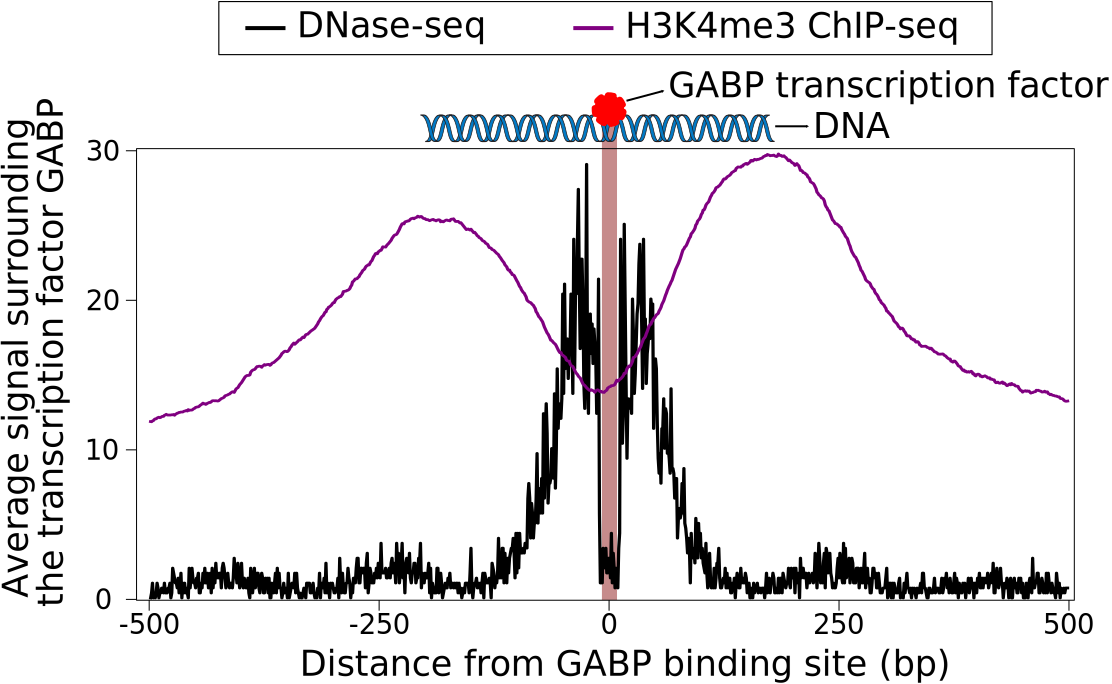
\includegraphics[width=0.8\textwidth]{gusmao_tfbs_pattern}
\caption[Distinctive pattern of DNase-seq and ChIP-seq on active TFBSs]{\textbf{Distinct pattern of DNase-seq and ChIP-seq on active TFBSs.} In this figure we show the average DNase-seq and histone modification H3K4me3 ChIP-seq signals surrounding the transcription factor GABP active binding sites. Active transcription factor binding sites happen at depletions between two peaks of the DNase-seq signal. Furthermore, these DNase-seq peaks, which determines an open chromatin region, happen at the depletion between two peaks of active histone modification marks.}
\label{fig:gusmao_tfbs_pattern}
\end{figure}

%%%%%%%%%%%%%%%%%%%%%%%%%%%%%%%%%%%%%%%%%%%%%%%%%%%%%%%%%%%%%%%%%%%%%
% Section: Contributions
%%%%%%%%%%%%%%%%%%%%%%%%%%%%%%%%%%%%%%%%%%%%%%%%%%%%%%%%%%%%%%%%%%%%%
\section{Contributions}
\label{sec:contributions}

% Framework to analyze footprints
The main contribution of this work is the development of a novel computational framework to treat data generated with the DNase-seq and ChIP-seq technologies and a novel computational method to detect active transcription factor binding sites based on these data. We developed a novel computational method to detect active TFBSs using the probabilistic framework of hidden Markov models. We performed in-depth investigations on issues related to the computational identification of active transcription factor binding sites, such as:

\begin{itemize}
\item Empirical analyses on the parameter selection of our methodology to perform optimal prediction of active transcription factor binding sites.
\item Correction of experimental artifacts introduced by the biological and computational protocols to generate DNase-seq and ChIP-seq data.
\item Optimal metrics to score and rank computational predictions of active transcription factor binding sites.
\item Identification of problematic transcription factors, in which the prediction is difficult given their very low binding residence time on the DNA.
\end{itemize}

% Extensive literature overview and method comparison
We evaluated ours and competing methods in multiple data sets available from public repositories. We evaluated the methods using the traditional approach based on ChIP-seq for TFs. Furthermore, we developed a novel evaluation methodology which includes gene expression instead of ChIP-seq for TFs, avoiding potential biases introduced by the latter. Comprehensive statistical analyses were performed to compare: our novel computational framework, nine competing methods and four baseline approaches.

% Case studies
Finally, we successfully applied our novel computational framework to predict active transcription factor binding sites on real biological experiments. Our method assisted in the identification of the regulatory players involved in two different biological systems:
\begin{itemize}
\item The differentiation of dendritic cells.
\item The inflammatory response of pancreatic Huvec cells.
\end{itemize}

%%%%%%%%%%%%%%%%%%%%%%%%%%%%%%%%%%%%%%%%%%%%%%%%%%%%%%%%%%%%%%%%%%%%%
% Section: Document Structure
%%%%%%%%%%%%%%%%%%%%%%%%%%%%%%%%%%%%%%%%%%%%%%%%%%%%%%%%%%%%%%%%%%%%%
\section{Document Structure}
\label{sec:document.structure}

% Chapter 2
In Chapter~\ref{cha:background} we introduce all the concepts needed for the understanding of our work. We clearly define the DNase-seq and ChIP-seq techniques. The problem we are addressing -- the computational identification of active TFBSs -- is clearly stated and a comprehensive literature review on computational methods to detect active transcription factor binding sites is performed.

% Chapter 3
In Chapter~\ref{cha:methods} we formalize all methods used in our analyses. We describe the treatment of the input DNase-seq and ChIP-seq data and the novel approach to detect active TFBSs based on hidden Markov models.

% Chapter 4
In Chapter~\ref{cha:experiments} we describe the full experiment design of this project. We present all the data used in our work. After, we describe the execution of our computational approach to detect active TFBSs. Then we describe the standard literature evaluation methodology (based on TF ChIP-seq) and a novel evaluation methodology based on gene expression. Finally, we describe the execution of all competing methods analyzed in this thesis.

% Chapter 5
In Chapter~\ref{cha:results} we present the results of our experiments. The results are grouped under the categories:
\begin{itemize}
\item Empirical analysis to select optimal parameters for our computational framework.
\item Investigation of footprint scoring strategies and the impact on performance of experimental biases.
\item Impact on performance of the issue regarding the transcription factor residence time.
\item Comprehensive comparative study involving $14$ different computational methods to predict active TFBSs.
\item Example of a common downstream analysis -- the \emph{de novo} motif finding based on the predicted active TFBSs.
\item Two case studies in which our predicted active TFBSs were used to identify the regulatory players involved in different biological conditions.
\end{itemize}

% Chapter 6
In Chapter~\ref{cha:concluding.remarks} we summarize all contributions performed by this research project, highlighting all the key findings. Furthermore, we discuss the future research opportunities which follows from the work presented in this thesis. Further supplementary results, figures and tables can be found in the Appendix~\ref{cha:appendix}.


